\documentclass[a4paper, 12pt]{article}
\usepackage[T1]{fontenc}
\usepackage[utf8]{inputenc}
\usepackage{apacite}
\usepackage{mathptmx}
\usepackage{enumerate}
\usepackage[margin=0.5in]{geometry}
\usepackage{xspace}
\usepackage{booktabs}
\usepackage{tabularx}
\usepackage{graphicx}

\renewcommand{\baselinestretch}{1.0}

\newcommand\nd{\textsuperscript{nd}\xspace}
\newcommand\rd{\textsuperscript{rd}\xspace}
\newcommand\nth{\textsuperscript{th}\xspace} %\th is taken already

\setlength\parindent{0pt} % set paragraph indent to zero

% fill up your name, ID, contribution and paper title here
\author{
Nurdiyana Athirah Binti Abdul Karim \quad 241UC2407E \quad Research Proposal \\
Ahmad Adam Affnan Bin Rozainey \quad 241UC240C7 \quad Research Proposal\\
Karthekeyan \quad 1211108235 \quad Presentation Slides\\
Sinehaa A/P Paramasivam \quad 1211103116 \quad Presentation Slides\\
}
\title{ Addressing Integration Challenges of Consensus Protocols and Verification Techniques within Layered Blockchain Frameworks  }

\begin{document}
\maketitle

\section*{Executive Summary}
As blockchain technology evolves quickly, it's clear that we need strong security frameworks to tackle its complex vulnerabilities. Unfortunately, many current solutions are disjointed and fail to effectively connect consensus protocols and verification techniques in layered blockchain systems. This research will explore the challenges of integrating these elements to improve the resilience of blockchain networks against new cyber threats.\\

This study has three main goals. First, it aims to create a comprehensive blockchain security framework that brings together layered architecture, consensus protocols, and formal verification methods. Second, it will assess the scalability and implementation challenges of incorporating new consensus protocols, like Proof of Adjourn (PoAj), \cite{sayeed} and formal verification in real-world blockchain settings. Finally, the research will investigate how effective quantum-resistant cryptography can be when integrated into the layered framework to help address potential future threats.
This research proposal will incorporate a mixed-methods approach, combining qualitative and quantitative analyses. Beginning with a comprehensive literature review to identify best practices and gaps in existing frameworks. The integration framework will be designed based on theoretical foundations and then tested in controlled environments to assess scalability and performance. Simulated quantum attacks will be conducted to evaluate the effectiveness of quantum-resistant cryptographic methods. Data will be collected through experiments, simulations, and performance metrics to support the analysis.\\

This research aims to develop a unified blockchain security framework that integrates layered architecture with consensus protocols and verification techniques. Additionally, it will produce a detailed report examining the scalability and implementation challenges of combining Proof of Adjourn (PoAj) and verification methods, including performance metrics and practical recommendations. Lastly, the research will evaluate quantum-resistant cryptographic methods tailored for blockchain applications, providing guidelines for their effective implementation. By offering an integrated framework, this study aims to enhance the resilience of blockchain systems against existing and emerging threats, including quantum computing. The findings will offer valuable insights for blockchain developers, policymakers, and researchers, contributing to the development of secure and future-proof blockchain solutions. Additionally, this research will pave the way for further exploration of integrated security approaches, thereby fostering innovation and confidence in blockchain technology across various industries.
\cite{kushwaha}.
\hfill
\\
\\
\textbf{Keywords:} Blockchain technology, Security frameworks, Consensus protocols, Verification techniques, Layered architecture, Proof of Adjourn (PoAj), Quantum-resistant cryptography, Integration challenges, Scalability, Implementation challenges, Qualitative analysis, Quantitative analysis, Literature review, Theoretical foundations, Controlled environments, Simulated quantum attacks, Performance metrics, Blockchain resilience, Cyber threats, Future-proof solutions, Integrated security approaches, Blockchain developers, Policy implications \\

\section{Introduction}
Blockchain technology has completely revolutionised digital transactions and data sharing in an array of industries due to its decentralised framework and secure features. But as blockchain systems become larger and more intricate, the security issues they encounter becomes more complex. Ensuring the stability of these networks is now of vital significance, especially in view of the emergence of modern threats such as quantum computing and more sophisticated attacks. Protocols for consensus and verification techniques have been developed as solutions, though current approaches often lack the consistency needed to fully secure blockchain networks.\\

Blockchain technology has completely revolutionised digital transactions and data sharing in an array of industries due to its decentralised framework and secure features. But as blockchain systems become larger and more intricate, the security issues they encounter becomes more complex. Ensuring the stability of these networks is now of vital significance, especially in view of the emergence of modern threats such as quantum computing and more sophisticated attacks. Protocols for consensus and verification techniques have been developed as solutions, though current approaches often lack the consistency needed to fully secure blockchain networks.\\

One major concern is the combination of consensus protocols, which control formal verification procedures which verify the system's accuracy and security. With a variety of consensus being developed such as Proof of Work (PoW), Proof of Stake (PoS), on top of the newer models like Proof of Adjourn (PoAj), they are typically used in isolation. Formal verification methods, which are essential for detecting vulnerabilities similarly are not fully integrated into blockchain architecture. Blockchain undermines their potential to offer complete protection throughout the layered structure of blockchain systems as the security solutions are disconnected.

The fragmented solutions reveal a critical research gap: the need for an integrated approach that unites consensus protocols, formal verification techniques, and layered blockchain architectures into a cohesive framework. Ultimately, addressing integration vulnerabilities is vital in ensuring the blockchain systems security in the long run due to the emergence of threats such as quantum computing. \\

This research will look into the challenges of incorporating consensus protocols and verification techniques within a layered structure of the blockchain, with a focus to improve scalability and security against emerging threats and attacks. This study aims to develop a comprehensive structure that enhances the overall security of blockchain's framework. \\

By addressing these issues, This research seeks to contribute valuable insights and findings that will help blockchain developers, regulators and researchers secure blockchain systems against any current and future threats by addressing practical implementation challenges.
 \\
 \cite{Hossain}.


\section{Problem Statement}
Blockchain technology offers decentralized and secure solutions across many industries, but it still faces several Cybersecurity challenges. One major issue is the lack of coordination between security measures, especially when it comes to combining consensus protocols and formal verification techniques within the layered blockchain frameworks. Consensus protocols like Proof of Work (PoW) and Proof of Stake (PoS) are important to maintain the integrity of blockchain by ensuring all participants agree on the state of the network. On the other hand, formal verification techniques are used to thoroughly check smart contract code, helping improve security in blockchain applications.
The problem is that these security mechanisms often operate separately, creating gaps in the system’s overall defense. The integration of new protocols, like Proof of Adjourn (PoAj), along with formal verification, into the seven-layer blockchain architecture hasn’t been fully explored. Additionally, emerging risks such as quantum computing add to the complexity, emphasizing the need for solutions like quantum-resistant cryptography to secure blockchain systems in the future. \\
This fragmentation leads to some key challenges:
\\
Scalability Problems: Combining consensus protocols like PoAj with verification techniques can slow down performance, especially when handling large numbers of transactions. 
\\
Implementation Difficulties: Incorporating these security measures into blockchain systems is often tricky due to compatibility issues with existing setups and the challenge of getting network participants to adopt them.
\\
New Threats: As quantum computing advances, blockchain systems will require quantum-resistant solutions, but these haven't been fully integrated with current consensus and verification methods yet.

\section{Research Questions, Hypotheses and Objectives}
\subsection{Research Questions:}
- How can consensus protocols and formal verification techniques be integrated into a layered blockchain security framework to enhance overall system resilience?
\\
- What are the key scalability and implementation challenges when integrating novel consensus protocols, such as PoAj, into existing blockchain systems?
\\
- How can a multi-layered blockchain security framework be optimized to address emerging threats such as quantum computing?

\subsection{Hypotheses:}
- H1: Integrating consensus protocols with formal verification techniques within a layered blockchain framework will enhance the overall security and reduce the risk of attacks, such as selfish mining and reentrancy, compared to implementing them separately.
\\
- H2: The adoption of quantum-resistant cryptography, when integrated with existing consensus protocols, will improve the blockchain system’s resilience against future quantum-based threats without significantly impacting performance.
\\
- H3: A well-integrated system combining novel consensus protocols (e.g., PoAj) with formal verification techniques can maintain scalability and performance, even under high transaction volumes, compared to existing standalone implementations.

\subsection{Research Objectives:}
\begin{enumerate}
    \item To develop an integrated blockchain security framework that combines layered architecture, consensus protocols, and formal verification methods.
    \begin{itemize}
    \item Specific: Create a framework combining PoAj and formal verification techniques within a layered architecture.
    \item Measurable: Success will be measured by the reduction of identified vulnerabilities across blockchain layers.
    \item Achievable: The objective will focus on integrating existing frameworks and protocols rather than developing new ones.
    \item Realistic: The objective leverages existing blockchain technologies while addressing their gaps.
    \item Time-bound: The integration framework will be completed within 12 months.
\end{itemize}

     \item To evaluate the scalability and implementation challenges of integrating PoAj and formal verification in real-world blockchain environments.
     \begin{itemize}
    \item Specific: Analyze performance and scalability issues of PoAj under high transaction volumes.
    \item Measurable: Scalability will be measured using transaction throughput, latency, and network disruption metrics.
    \item Achievable: Testing will focus on controlled environments and test networks before live blockchain deployment.
    \item Realistic: Given that PoAj has theoretical foundations, the evaluation will explore practical implementation.
    \item Time-bound: Evaluation and reporting will be completed within 6 months.
\end{itemize}

     \item To explore the effectiveness of quantum-resistant cryptography within the layered framework for mitigating future threats.
     \begin{itemize}
    \item Specific: Investigate quantum-resistant methods in the Data and Network layers of the blockchain framework.
    \item Measurable: Effectiveness will be measured through simulated quantum attacks and vulnerability assessments.
    \item Achievable: Focus will be on existing quantum-resistant techniques like lattice-based cryptography.
    \item Realistic: The research builds on current cryptographic advancements and applies them to blockchain systems.
    \item Time-bound: Testing and analysis will be completed within 9 months.
\end{itemize}
\end{enumerate}

\section{Literature Review}
Blockchain technology evolves day by day, resulting in various research efforts being done to explore different perspectives to enhance its security. Existing studies highlight consensus protocols, formal verification method, and blockchain security frameworks. Although, a recurring theme is the fragmented approach in solving the vulnerabilities of blockchain security, particularly to integrate these components into a cohesive system.\\

A significant aspect of study is the multi-layered blockchain security architectures development. These architectures offer an approach that is more flexible to secure different elements of blockchain systems. Despite their strength in theory, the scalability and applicability of these framework remain uncertain, as these proposals lack validation in real-world scenarios.\\

Another major emphasis is the integration of formal verification techniques into blockchain systems. These methods are crucial in detecting and avoid any vulnerabilities. However, these techniques have been discussed in existing studies, neglecting their broader utility within a multi-layered system. In addition to that, the high level of computation and formal methods of authentication resource demands raise concerns regarding their adaptability, particularly in blockchain settings that are more complex.\\

As the blockchain industry evolves, quantum computing emerges as a major potential threat with the capability to undermine established methods of encryption. Several studies suggest that quantum-resistant cryptographic approaches as possible defences against any cyber attacks. However, the practical application of these quantum-resistant approaches into multilayer blockchain architectures has not been thoroughly investigated. Current research lacks real performance data, notably in terms of scalability and the effectiveness of these strategies against simulated quantum attacks.\\

Consensus protocols such as Proof of Adjourn (PoAj), have been proposed to improve blockchain scalability and energy efficiency. There is a lack of studies on the practical implementation, even though these protocols offer creative solutions. Specifically, the challenges of deploying PoAj in high-transaction blockchain environments, as well as its integration with other security mechanisms like formal verification and cryptography, remain unaddressed.\\

A significant gap identified across the literature is the lack of integration across an array of blockchain security solutions. While much attention has been paid to isolated aspects such as consensus protocols, cryptographic methods, and verification techniques, there is a lack of studies on how to integrate these components into a unified, multi-layered system. This fragmentation leaves blockchain systems vulnerable to emerging threats and limits their ability to scale securely.//

\section{Research Methodology}
This research adopts a mixed-methods approach, combining both qualitative and quantitative methodologies to develop and evaluate a robust blockchain framework that integrates consensus protocols and verification techniques. The following steps outline the approach, with evaluation metrics and techniques applied at each stage.
\begin{enumerate}
    \item \textbf{Comprehensive Literature Review}
\begin{itemize}
    \item Identify existing frameworks: Explore consensus protocols and verification techniques currently used in blockchain.
    \item Highlight research gaps: Pinpoint deficiencies, such as scalability challenges, performance issues, and integration difficulties in current approaches.
\end{itemize}

    \item \textbf{Framework Design and Development}
\begin{itemize}
    \item Based on the insights gained from the literature review, a layered blockchain integration framework will be designed. This framework will ensure a secure, scalable, and efficient blockchain system by integrating:
     \item Consensus protocols: Traditional proof-based systems and emerging quantum-resistant methods.
      \item Verification techniques: Formal verification methods, including static code analysis and mathematical proofs for smart contract validation.
\end{itemize}

\item \textbf{Controlled Environment Testing}
\\
The framework will be implemented in a controlled blockchain testnet environment. The following algorithms and protocols will be employed:
\begin{itemize}
    \item Consensus Protocols: Proof of Work (PoW), Proof of Stake (PoS), and novel approaches such as Proof of Adjourn (PoAj).
    \item Verification Techniques: Formal verification (e.g., symbolic execution), gas cost estimations, and runtime verification tools to assess vulnerabilities in smart contracts.
    \item Quantum-Resistant Methods: Integration of quantum-resistant cryptographic algorithms (e.g., Lattice-based encryption).
\end{itemize}

\item \textbf{Simulated Quantum Attacks}
\\
Quantum-resistant cryptography will be subjected to simulated quantum attacks using post-quantum cryptographic techniques. Attack simulations will assess how resistant the proposed framework is to these evolving threats.

\item \textbf{Data Collection and Performance Metrics}
\\
Data will be collected through simulations and experiments to measure the framework’s effectiveness across various domains:
\begin{itemize}
    \item Scalability: Measured by transaction processing rate (TPS), latency, and network throughput under varying loads.
    \item Security: Evaluated by the framework’s resistance to known and emerging attack vectors, including selfish mining and quantum-based attacks.
    \item Efficiency: Assessed by computational cost, energy consumption, and resource usage.
    \item Resilience: How well the system adapts to and recovers from new attack vectors or vulnerabilities.
\end{itemize}

\begin{table}[htbp]
    \centering
    \begin{tabular}{|p{3cm}|p{8cm}|p{5cm}|}
        \hline
        \textbf{Metric} & \textbf{Description} & \textbf{Measurement} \\ \hline
        Scalability & Measures the ability to handle high transaction loads effectively. & Transactions per second (TPS) \\ \hline
        Performance & Evaluates the speed and efficiency of the integrated framework. & Latency in milliseconds \\ \hline
        Security & Assesses the system's effectiveness against attacks. & Success rate of attacks \\ \hline
        Implementation Complexity & Evaluates challenges in adopting the framework. & Deployment time in hours \\ \hline
        Quantum Resistance & Tests the system's ability to resist quantum attacks. & Success rate of quantum attack simulations \\ \hline
    \end{tabular}
    \label{tab:evaluation_metrics}
    \caption{Key Evaluation Metrics for Blockchain Framework}
\end{table}

\item \textbf{Data Analysis}
\begin{itemize}
    \item Quantitative Data: Metrics from the performance analysis (scalability, security, efficiency) will be statistically evaluated. Tools such as performance graphs and statistical correlation analyses will be used to evaluate the robustness of the framework.
    \item Qualitative Feedback: Insights from testing environments will reveal any practical implementation challenges, user experience issues, and unforeseen system limitations.
\end{itemize}

\end{enumerate}

\textbf{Models and Algorithms}
\begin{itemize}
    \item Consensus Protocols: PoW, PoS, PoAj, and quantum-resistant consensus methods will be compared.
    \item Formal Verification Methods: Symbolic execution for smart contract validation.
    \item Quantum-Resistant Cryptography: Algorithms such as Lattice-based encryption will be employed to protect the blockchain against quantum attacks.
\end{itemize}
\cite{MARIJAN}.

\newpage

\section{Research Findings and Milestones}

\begin{figure}[htbp] % 'htbp' allows flexibility in figure placement
    \centering
    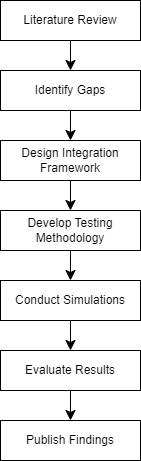
\includegraphics[width=0.2\linewidth]{flowchartresearch.jpg} % Adjust width as needed
    \caption{Research Activities}
    \label{fig:research_activities} % Updated label for clarity
    
    \vspace{1cm} % Adds vertical space between images
    
    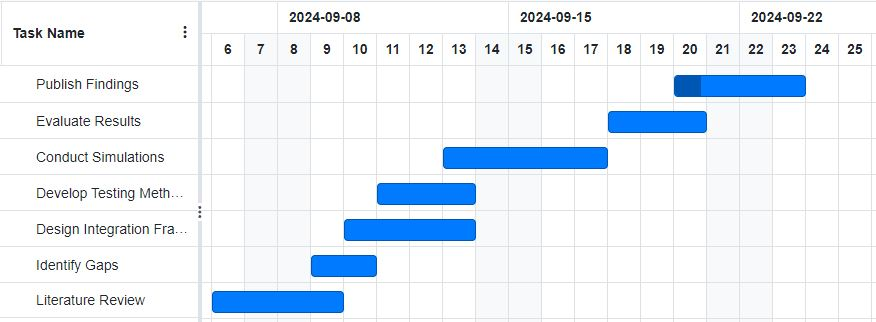
\includegraphics[width=0.8\textwidth]{ganttresearch.jpg} % Adjust width as needed
    \caption{Research Schedule}
    \label{fig:research_schedule} % Updated label for clarity
\end{figure}

\newpage
\section{Expected Results and Impact}
\textbf{Novel Theories and Findings}
\\
Improved Integration Framework: The creation of a detailed integration framework will offer a structured way to combine different consensus protocols and verification techniques. This new framework aims to tackle the current issues around scalability and security, making blockchain systems stronger and more reliable.
\\
Quantum-Resistant Cryptography: By including quantum-resistant cryptographic techniques, this research will create frameworks that protect blockchain systems from future quantum computing threats. This progress will help ensure that blockchain technology remains dependable as quantum attacks become more possible.
\\
Evaluation Metrics for Frameworks: The introduction of specific metrics to assess the performance and security of blockchain frameworks will give researchers and industry professionals better tools for analysis. This could lead to more standardized ways of evaluating and applying blockchain technologies across the field.
\\
\\
\textbf{Impact on Society}
\\
Increased Trust and Security: By enhancing the security features of blockchain systems, this research will foster greater trust among users, especially in sectors like finance, healthcare, and supply chain management. This trust is essential for wider adoption of blockchain technologies, which could revolutionize transaction methods and data integrity.
\\
Empowerment of Individuals and Businesses: As blockchain systems become more secure and efficient, individuals and small businesses will gain more access to decentralized financial services and applications, reducing reliance on traditional banking systems. This empowerment could lead to increased financial inclusion and economic opportunities for underserved communities.
\\
\\
 \textbf{Impact on the Nation}
Strengthening National Security: By developing robust frameworks that protect against emerging cyber threats, this research contributes to national security. Secure blockchain systems can safeguard sensitive information and ensure the integrity of governmental and financial operations, reducing the risk of cyberattacks.
\\
Supporting Innovation and Competitiveness: The findings from this research can help establish national standards in blockchain technology, encouraging innovation within the tech industry. A strong focus on security and scalability will position the nation as a leader in blockchain development, attracting investments and talent.
\\
\\
\textbf{Economic Impact}
\\
Stimulating Economic Growth: The adoption of improved blockchain technologies can streamline operations across various sectors, reducing costs and increasing efficiency. This efficiency can drive economic growth as businesses benefit from lower transaction fees and faster processing times.
\\
Job Creation in Tech Sector: As blockchain technologies evolve and require more sophisticated integration frameworks, new job opportunities will arise in fields such as cybersecurity, software development, and data analysis. This research can thus contribute to job creation and workforce development in the tech sector.
%References
\bibliographystyle{apacite}
\bibliography{MyBib}{}


\end{document}

